\section{Resonance \label{sec:res}}
Using resonances inside a tube to measure the velocity of second sound.
A signal generator heats superfluid in a tube and acts as a reference signal
to the phase detector. An Allen-Bradley (AB) resistor measures the fluctuations
of temperature of the other side of resonance tube, when the two are
in phase, resonance is set up a measurable frequency.

\subsection{Theory}
\begin{figure}[htbp]
\centering
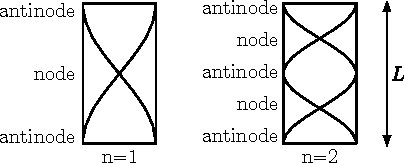
\includegraphics{pics/harmonicsintube.pdf}
\caption{Harmonics forming inside the resonance chamber of the cryogenic environment \label{fig:harmonicsintube}}
\end{figure}
Inside the resonance tube the second sound resonates down the length $L$, Figure \ref{fig:harmonicsintube}.
For a wavelength $\lambda$, and harmonic $n$.
The fundamental frequency at $n=1$ is $\lambda / 2$. Generalizing for n, Equation \ref{equ:lny2}.
\begin{equation}
L = \frac{n \lambda_n}{2} \to \lambda_n = \frac{2L}{n} \label{equ:lny2}
\end{equation}
The velocity from the standard wavelength frequency relation $v=f\lambda$ can be
rearranged for $\lambda$ with $\lambda = \lambda_n$ and $f = f_n$ to get Equation \ref{equ:v2fln}.
\begin{equation}
v = f_n\lambda_n \to v = 2f_n \frac{L}{n} \label{equ:v2fln}
\end{equation}

The heating that adds entropy and temperature for the second sound waves 
comes for a coil heater connected to a signal generator.
The heating requires a bit more theory connecting
the power of the coil to the current applied.
The heating coil works with ohmic heating, Equations \ref{equ:piv}, \ref{equ:vir}.
\begin{equation}
P=IV \label{equ:piv}
\end{equation}
\begin{equation}
V=IR \label{equ:vir}
\end{equation}
And as \ref{equ:vir}, get to
the recognisable result \ref{equ:pi2r}:
\begin{equation}
\label{equ:pi2r}
P=I^2 R
\end{equation}
The current $I$ from the signal generator is varied
according to:
\begin{equation}
\label{equ:wavegenneratorI}
I = I(t) = I_0 \cos(\omega t)
\end{equation}
So from \ref{equ:pi2r}
\begin{equation}
\label{equ:wavepower1}
P = P(t) = I_0^2  \cos^2(\omega t) R
\end{equation}
Using the double angle relation
\begin{equation}
\label{equ:doubleangle1}
\cos(2\theta) = 2 \cos^2(\theta) - 1
\end{equation}
Re-arranged for $\cos^2(\theta)$:
\begin{equation}
\label{equ:doubleangle2}
\cos^2(\theta) = \frac{1 + \cos(2 \theta)}{2}
\end{equation}
With Equations \ref{equ:wavepower1} and \ref{equ:doubleangle2}
and setting $\theta = \omega t$ then:
\begin{equation}
\label{equ:powerequation}
P = \frac{I_0^2 R^2}{2} \left( 1 + \cos(2\omega t)\right)
\end{equation}
By observing the term inside cos() the heating frequency
($\omega_P$ power) is twice the drive frequency ($\omega_I$ current).
\begin{equation}
\label{equ:powercurrrentfrequencyrel}
\omega_P = 2 \omega_I
\end{equation}
This means that:
\begin{equation}
\label{equ:gennyfreqheatfreq}
f_n = 2 f_\text{gennerator}
\end{equation}
The frequency for the harmonic is twice the frequency used to drive the heating
coil, for $f_\text{gennerator}$ as the generator frequency.
This is heat being produced from the coil for both forwards and backwards current,
two peaks of heat for one peak of current, as shown in Figure \ref{fig:pirelation}.

%%diagram showing the power and current frequencys.
\begin{figure}[htbp]
\centering
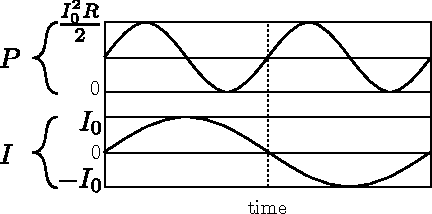
\includegraphics{pics/pirelation.pdf}
\caption{The power and current frequencys showing a factor of two gain in frequency.\label{fig:pirelation}}
\end{figure}

For $v$ as the propagation velocity from Equation \ref{equ:v2fln} above, it means that.
\begin{equation}
v = 2 f_n \frac{L}{n}
\end{equation}
is also
\begin{equation}
v = 4 f_\text{gen} \frac{L}{n} \label{equ:v4fgln}
\end{equation}
for $n=1$
\begin{equation}
v = 4 L f_\text{gen}
\end{equation}

For a measurement of different harmonics $n$ and the corresponding 
frequency $f_\text{gen}$, the a linear plot of frequency against harmonic would be the
straight line:
\begin{equation}
\underbrace{f_\text{gen}}_\text{y} = \underbrace{\frac{ d f_\text{gen}}{dn} n}_\text{mx} + c
\end{equation}
so 
\begin{equation}
v = 4 L \frac{ d f_\text{gen}}{dn} \label{equ:v4ldfdn}
\end{equation}

\subsection{Experimental Detail}

The insert into the cryostat is built similarly to Figure \ref{fig:pseuphysicsview}
on page \pageref{fig:pseuphysicsview}.
Small obstructions in the resonance chamber are 
the AB resistor on the rod and the AB resistor on the side.
The equipment is orientated similarly to Figure \ref{fig:pseuphysicsview} with the heating coil
heating downwards towards the AB resistor for detection.

\begin{figure}[htb]
\centering
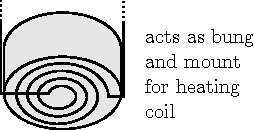
\includegraphics{pics/heatingbung.pdf}
\caption{Close-up view of the heat bung from Figure \ref{fig:pseuphysicsview} \label{fig:heatingbung}}
\end{figure}

The heating coil on the top is connected to the circuit and the coil is 
laid out on the inner surface to maximise a uniform heating surface, Figure \ref{fig:heatingbung}.

\begin{figure}[htb]
\centering
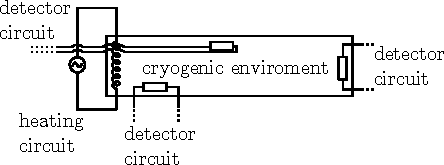
\includegraphics{pics/circuitconnections.pdf}
\caption{Circuit connection available to the cryogenic environment. \label{fig:circuitconnections}}
\end{figure}

The different components are attached to different circuits and are partly swappable,
a measurement of resistance can swap between any of the three AB resistors as in Figure \ref{fig:circuitconnections}.

\begin{figure}[htb]
\centering
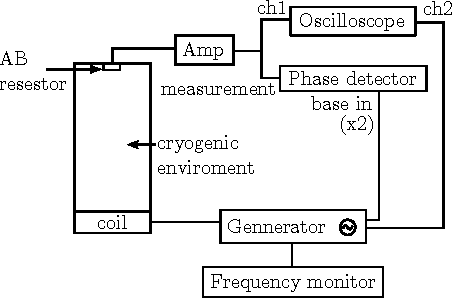
\includegraphics{pics/nodelayout.pdf}
\caption{Layout of the components connecting apparatus.  \label{fig:nodelayout}}
\end{figure}

For this experiment however the components are connected according to \ref{fig:nodelayout}.
The ``$\times 2$'' option is so that the Phase detector uses the effective heating frequency
and not just the current frequency as in Equation \ref{equ:gennyfreqheatfreq}.


The experiment is done at the coldest temperature available 
via pumping, 3.02 Tor.

%%stuff from lab book, 
%%needs splitting into outline theory expermental detial and results conclusion.
The frequency generator is connect to the heating circuit.
The detector circuit is connected to the lower AB resistor 
on the opposite face of the resonance chamber.
The frequency measurements are taken from a frequency monitor and represent $g_\text{gen}$.

A quick search for the first harmonic was conducted by changing the frequency of the
generator.
From this for scientific precision a range of values around that harmonic 
and the measurement of the in-phase detection was used to collected data around
the peak so that it can be evaluated more precisely.

Using the value for the first harmonic the second harmonic was looked for at
twice the fundamental frequency.
\begin{equation}
f_{n=2} = 2 f_{n=1}
\end{equation}
More data was taken around the range of the second harmonic in a similar manner
to the first.

For the later harmonics, $n = 3,4,5\ldots$, up to $n=7$, to reduce the
time of the experiment, a quicker method in real time conducted by the operator to
maximise the detected signal in
the phase signal analysis.
By looking for the jump of in-phase signal to find the harmonic,
then overshooting until a noticeably smaller in-phase signal and
moving back until no noticeable difference can be seen.
This process is shown in Figure \label{fig:tuningmethod}.

%diagram of live methd. 
\begin{figure}[htbp]
\centering
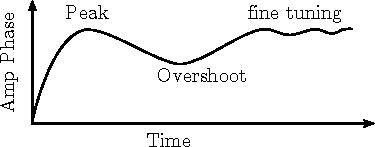
\includegraphics{pics/tuningmethod.pdf}
\caption{Sketch of `live' method used to find the peaks quickly. \label{fig:tuningmethod}}
\end{figure}

\subsection{Results}
The length of the tube for resonance is:
\begin{equation}
\boxed{ L = (72 \pm 1)\text{mm} }
\end{equation}

The first harmonic was found at around $72\pm5$Hz. 
The range of measurements around the fundamental yields Figure \ref{fig:firstharmonic}.
A Beta fitting function was added to find numerically the peak because it fits best with
the data. 
 
%table of results n=1 harmonic.
\begin{figure*}[htb]
\centering
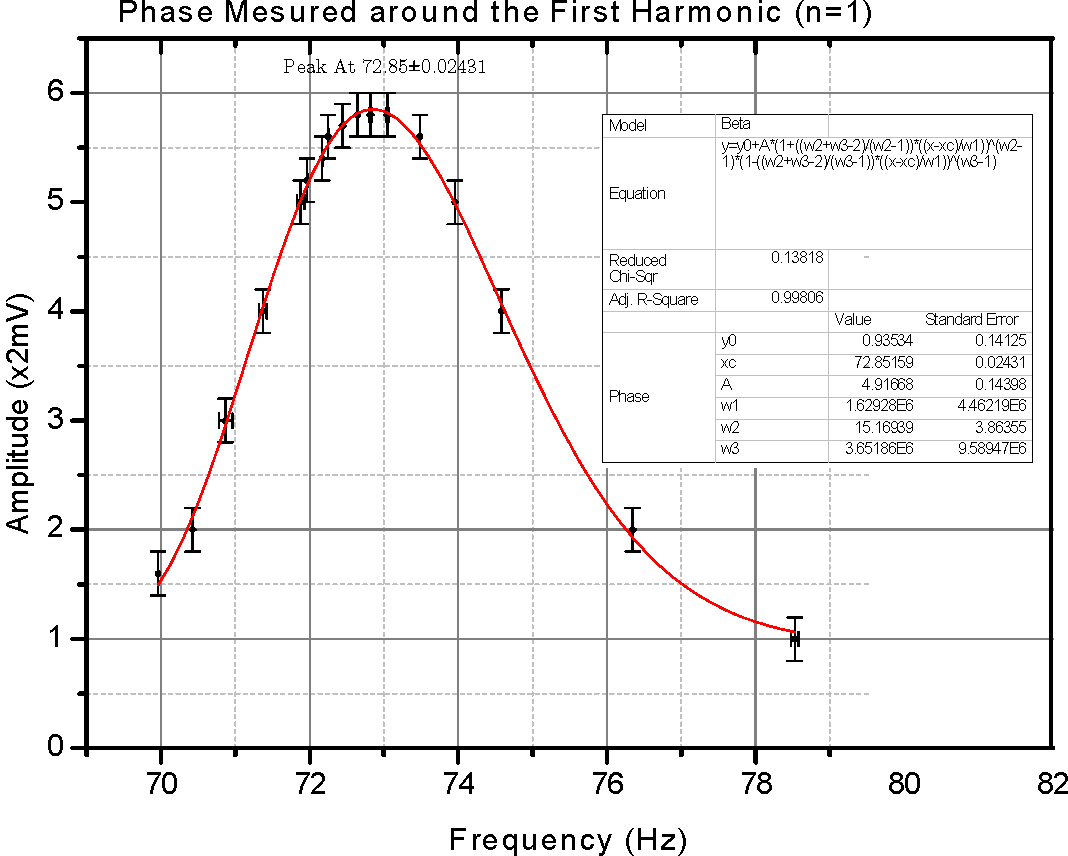
\includegraphics[width=0.8\textwidth]{pics/firstharmonic.pdf}
\caption{Amplitude and frequency around the first harmonic showing a peak at the resonance frequency. \label{fig:firstharmonic}}
\end{figure*}

From the graph the first harmonic is:
\begin{equation}
\boxed{ F_{n=1} = (72.852 \pm 0.024)\text{Hz}}
\end{equation}

This first peak shows some evidence for second sound in the superfluid.
%This peak fits with the theory of second sound.

The second harmonic search began at $\approx 140 $Hz.
Results of taking data yields Figure \ref{fig:secondharmonic2}.
The Lorentz fit works for points near to the peak.
However it does not fit all of the data well.
The fit is to wide at the sides and to narrow near the peaks centre.
But it does have a precise numerical value for the peak.

\begin{figure*}[htb]
\centering
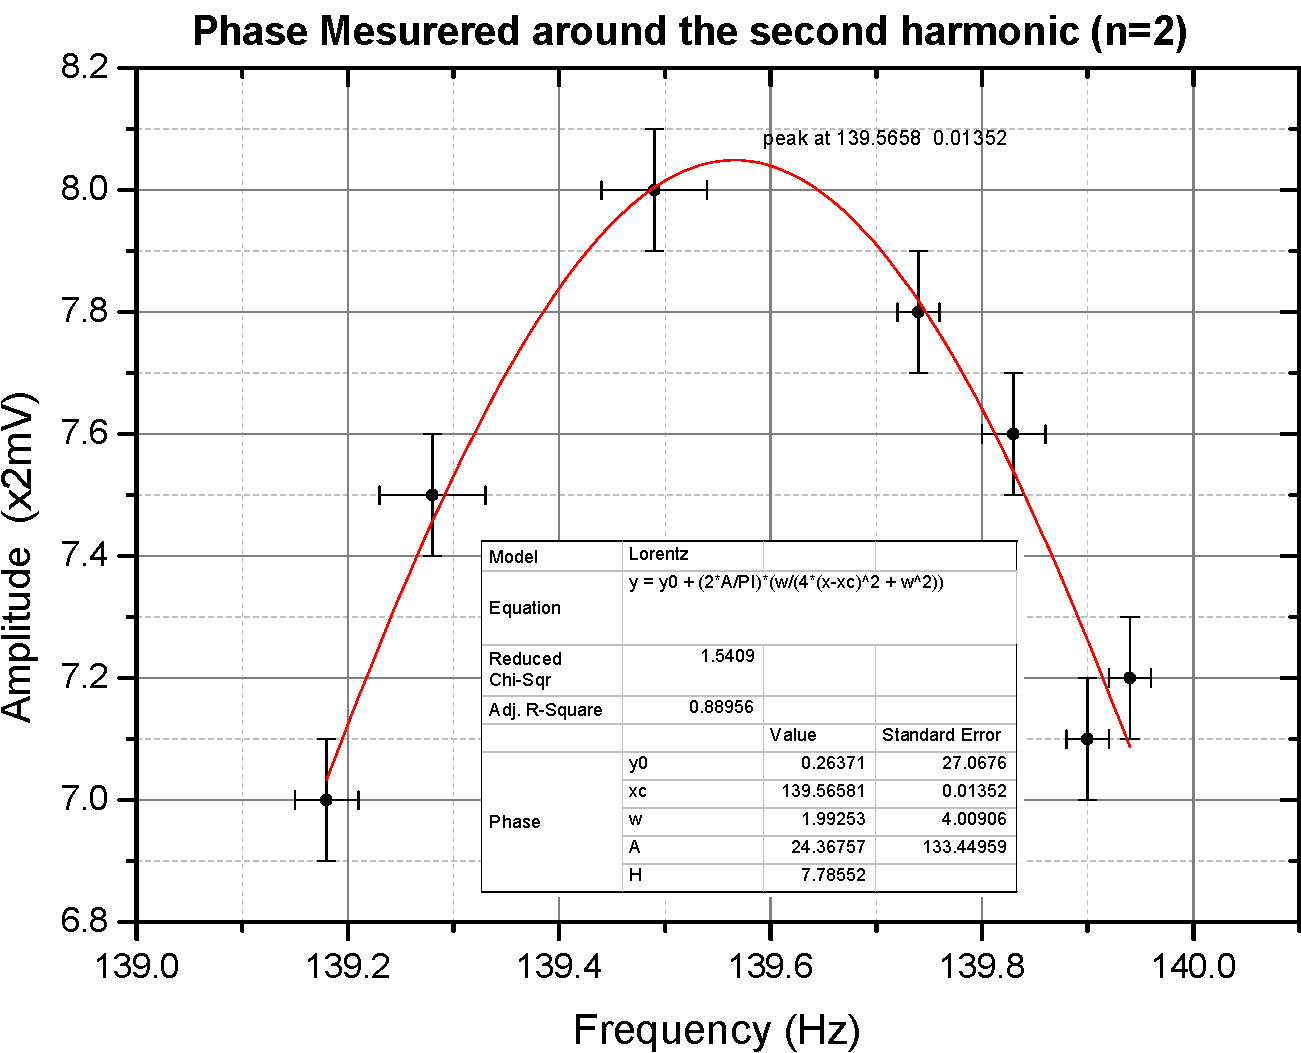
\includegraphics[width=0.8\textwidth]{pics/secondharmonic2.pdf}
\caption{Amplitude and frequency around the second harmonic showing a peak at the resonance frequency. \label{fig:secondharmonic2}}
\end{figure*}

%see log book  around n=2 results page..

The graph shows that the peak for the second harmonic is:
\begin{equation}
\boxed{f_{n=2} = (139.56 \pm 0.014)\text{Hz}}
\end{equation}

The remaining harmonics are found and recorded.
A table of the results up to n=7 is in the appendix in Table \ref{tab:harmonics}.

%%table of all n values.
The frequency of the harmonics of the second sound for a straight line when 
plotted against n. This agrees with Equation \ref{equ:v4ldfdn}.

A theoretical (0,0) point is added because of the logical extension of Equation \ref{equ:v4ldfdn}.

% n frequency graph.

\begin{figure*}[htb]
\centering
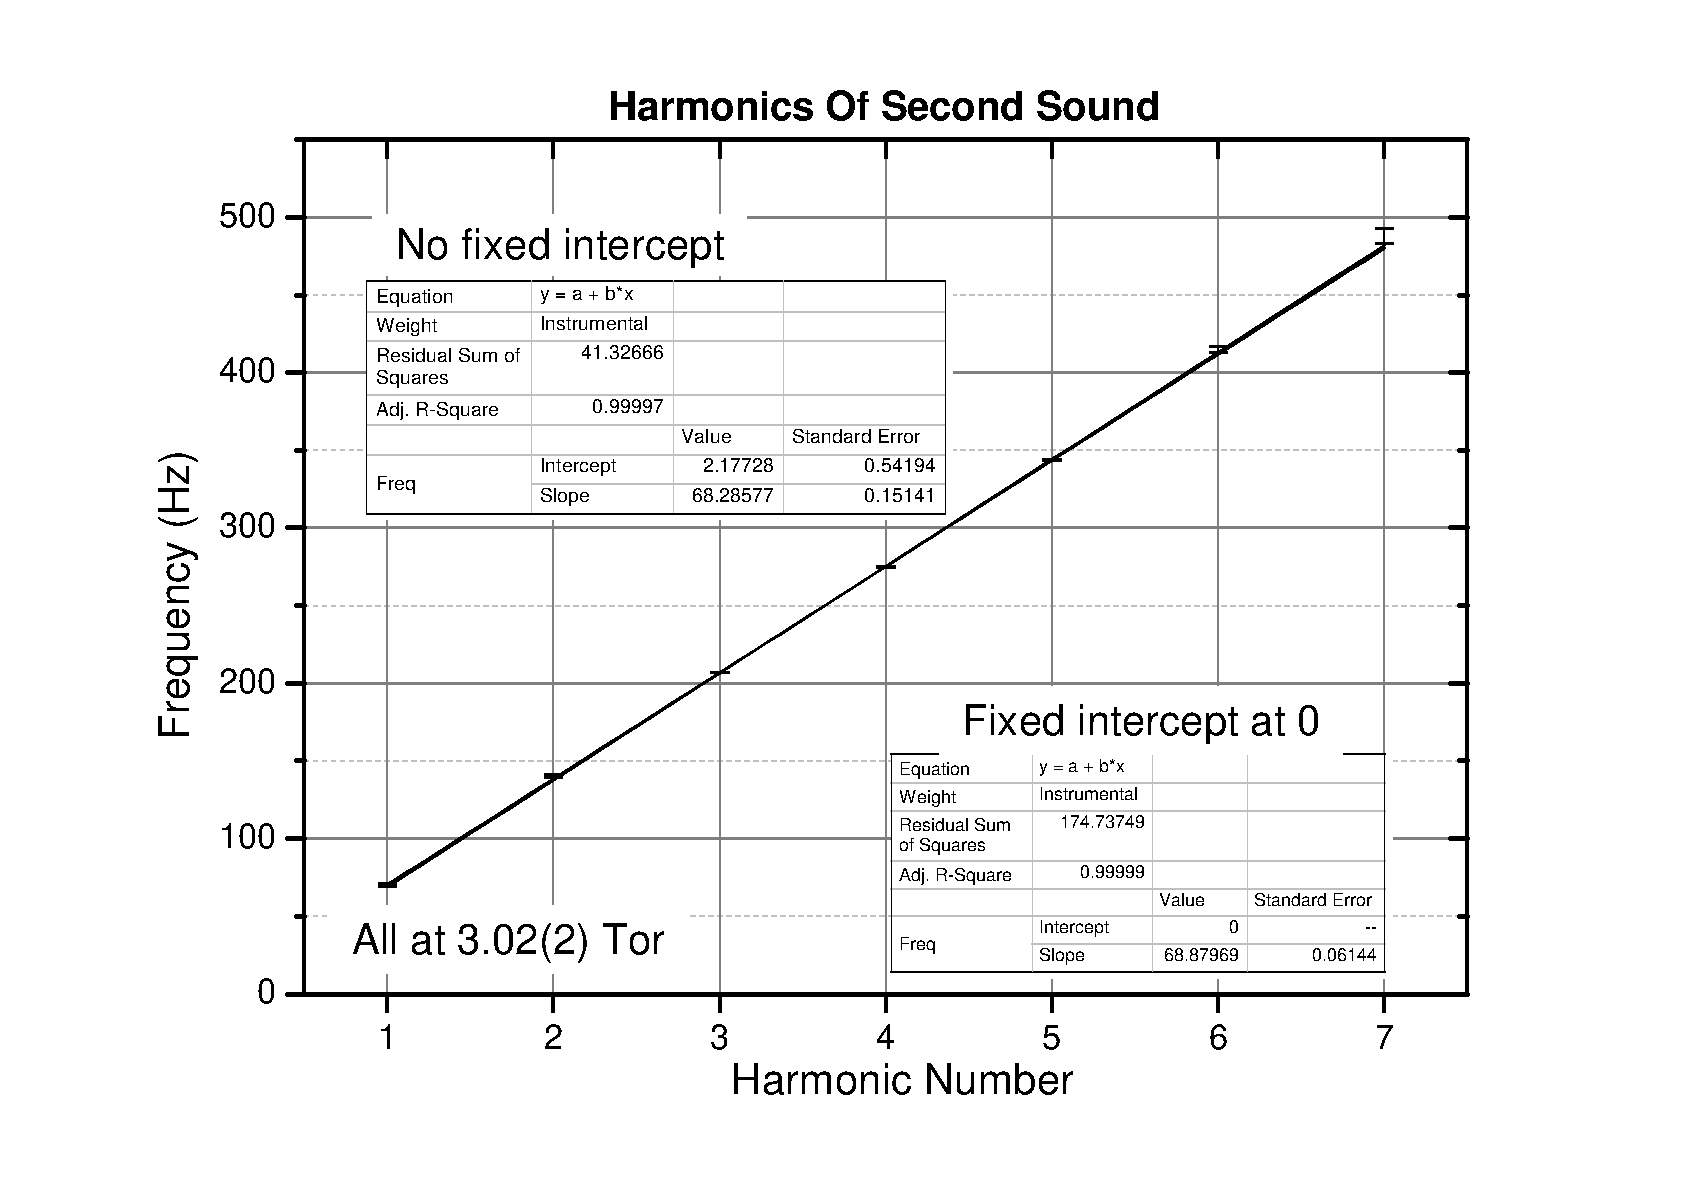
\includegraphics[width=0.8\textwidth]{pics/harmonicsofsecondsound.pdf}
\caption{The frequency of the generator and the harmonic\label{fig:harmonicsofsecondsound}}
\end{figure*}

The linear fit yields:
\begin{equation}
\boxed{\frac{df_n}{dn} = (68.879 \pm 0.061) \text{Hz}}
\end{equation}
the Intercept of 0 is included in the linear fit because the fitting is better.
The high values of $n = 6,7$ have a slight upwards curl, but the fitting weighting 
of the errors accounts for this.
The fitting still does not have an intercepts that covers 0.
This could be from the obstruction in the resonance tube or
none-uniform heating across the coil.

Using equation \ref{equ:v4ldfdn} with the measured value of $\frac{df_n}{dn}$ from the graph 
in Figure \ref{fig:harmonicsofsecondsound} to get:
\begin{equation}
\boxed{ v = (19.8372 \pm 0.2761) \text{ms}^{-1}}
\end{equation}
At 3.02 Tor.

\begin{figure*}[htb]
\centering
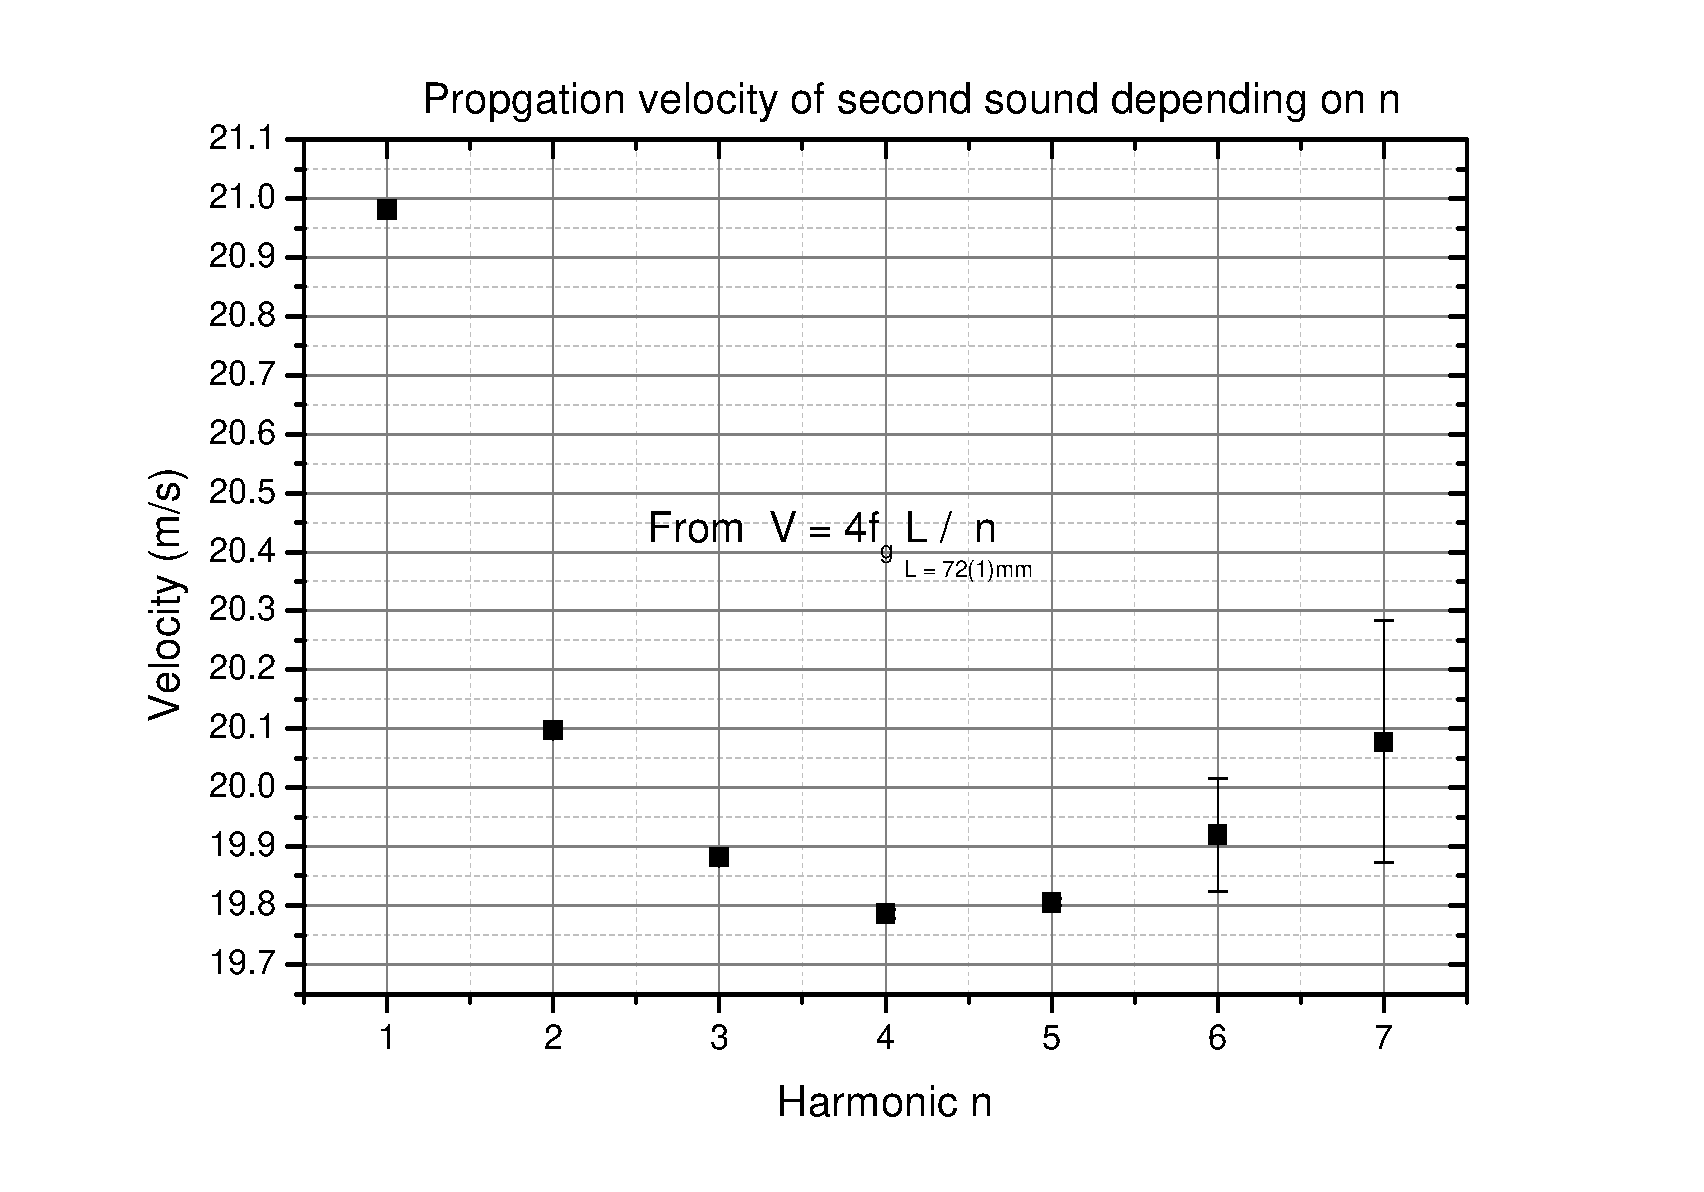
\includegraphics[width=0.8\textwidth]{pics/velocitydependingonn.pdf}
\caption{The frequency of the generator and the harmonic\label{fig:velocitydependingonn}}
\end{figure*}

An extra graph is produced using Equation \ref{equ:v4fgln}.
This uses the individual results (a less accurate method)
to calculate the apparent velocity at different harmonics,
something that should be constant.
However Figure \label{fig:velocitydependingonn} shows that 
the velocity changes with a `U' shaped curve with a minimum at 
$n=4$. The value for velocity calculated from $\frac{df_n}{dn}$
has uncertainty that cover the range from 19.56 to 20.11, this includes
all but the $n=1$ harmonic.
The $n=1$ harmonic is the most accurate measurement of the graph,
so there is another factor that is changing the calculated velocity.
It could be the heating from the coil that changes the temperature inside
the resonance tube so not all measurements of frequency were at the same
temperature, or it could be the wavelength that interferes with the
movable resistor at only certain lengths. 

\subsubsection{Observing Harmonics Shape}
As a qualitative exercise,
the movable resistor is hooked up to the phase detection circuit.
It is lowered starting from the upper position to the middle, then
from middle to the lower, Figure \ref{fig:variableresistormovement}.
The signal generator is set for the fundamental frequency.

It is not possible to get to the very top or very bottom of the resonance tube
because of physical limitations.

\begin{figure}[htb]
\centering
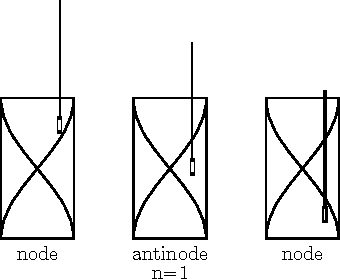
\includegraphics{pics/variableresistormovement.pdf}
\caption{The position of the movable resistor changing measuring
the \label{fig:variableresistormovement}}
\end{figure}

On the oscilloscope it is observed a node is in the
middle position and antinodes at the edges.

